\section{Introduction}

Smart contract vulnerabilities represent one of the most costly security challenges in modern computing. As shown in Figure~\ref{fig:losses}, cryptocurrency theft has resulted in over \$14 billion in losses since 2020, with 2025 already reaching \$3.4 billion, the highest since the 2022 peak \citep{chainalysis2025}. The Bybit breach alone accounted for \$1.5 billion, while the Cetus protocol lost \$223 million in minutes due to a single overflow vulnerability \citep{yellow2025}.

\begin{figure}[h]
\centering
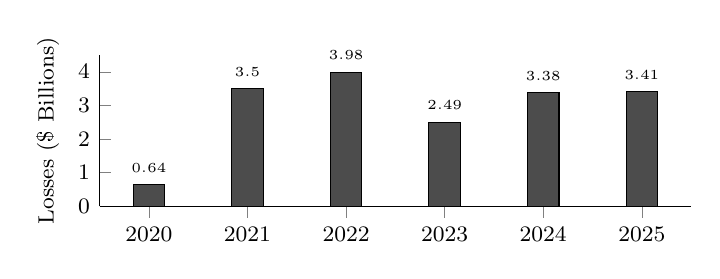
\begin{tikzpicture}
\begin{axis}[
    ybar,
    bar width=0.4cm,
    width=0.75\columnwidth,
    height=3.5cm,
    ylabel={Losses (\$ Billions)},
    ylabel style={font=\footnotesize},
    symbolic x coords={2020,2021,2022,2023,2024,2025},
    xtick=data,
    ymin=0,
    ymax=4.5,
    ytick={0,1,2,3,4},
    nodes near coords,
    nodes near coords style={font=\tiny, above},
    every node near coord/.append style={yshift=1pt},
    tick label style={font=\footnotesize},
    axis lines*=left,
    clip=false,
]
\addplot[fill=black!70] coordinates {(2020,0.64) (2021,3.5) (2022,3.98) (2023,2.49) (2024,3.38) (2025,3.41)};
\end{axis}
\end{tikzpicture}
\caption{Annual cryptocurrency theft losses (2020--2025). Data from Chainalysis.}
\label{fig:losses}
\end{figure}

Meanwhile, large language models have achieved remarkable success on programming tasks. Frontier models now pass technical interviews, generate production code, and identify bugs across diverse codebases. This raises a natural question: \textit{can these models apply similar expertise to blockchain security?} And if they can, \textit{are they genuinely reasoning about vulnerabilities, or merely pattern-matching against memorized examples?}

This distinction matters. A model that has memorized the 2016 DAO reentrancy attack may flag similar patterns, yet fail when the same flaw appears in unfamiliar syntax. We introduce \textbf{BlockBench}, a benchmark designed to answer this question. Our contributions include:

\begin{enumerate}[leftmargin=*, nosep]
    \item \textbf{BlockBench}, comprising 263 Solidity vulnerability samples with systematic contamination control and gold standard examples from recent professional security audits.

    \item \textbf{Composite evaluation metrics} distinguishing genuine understanding from memorization, validated through multi-configuration sensitivity analysis (Spearman's $\rho$=1.000).

    \item \textbf{Systematic assessment} revealing 58\% best-case detection on mixed samples collapsing to 20\% on uncontaminated professional audits, exposing heterogeneous robustness and accuracy-understanding gaps across models.

\end{enumerate}
